\documentclass[numbers=noenddot]{thesis}

% hier namen etc. einsetzen
\fullname{Fabian Fischbach, Luis Beaucamp und Tim Stenzel}
%\email{vorname.nachname@uni-ulm.de}
\headline{Mobile Application Development}
\titel{Thema}
\jahr{2017}
\matnr{Matrikel-Nr}
\gutachterA{Marc Schickler}
%\gutachterB{Gutachter 2}
\betreuer{Marc Schickler}
\typ{Ausarbeitung zur App "Coaster2Go" }
\fakultaet{Ingenieurwissenschaften, Informatik und \\Psychologie}
\institut{Institut für Datenbanken und Informationssysteme}

% Falls keine Lizenz gewünscht wird bitte den folgenden Text entfernen.
% Die Lizenz erlaubt es zu nichtkommerziellen Zwecken die Arbeit zu
% vervielfältigen und Kopien zu machen. Dabei muss aber immer der Autor
% angegeben werden. Eine kommerzielle Verwertung ist für den Autor
% weiter möglich.
\license{
This work is licensed under the Creative Commons.
Attribution-NonCommercial-ShareAlike 3.0 License. To view a copy of this
license, visit http://creativecommons.org/licenses/by-nc-sa/3.0/de/ or send a
letter to Creative Commons, 543 Howard Street, 5th Floor, San Francisco,
California, 94105, USA. \\ Satz: PDF-\LaTeXe
}

\hypersetup{%
	pdftitle=\pdfescapestring{\thetitel},
	pdfauthor={\thefullname},
 	pdfsubject={\thetyp},
}


% trennungsregeln
\hyphenation{Sil-ben-trenn-ung}

%-----------Pakete einfügen----------------
\usepackage{mwe}
\renewcaptionname{ngerman}{\figurename}{Abb.}


%------------------------------------------

\begin{document}
\frontmatter
\maketitle
% impressum
\clearpage
\impressum

\cleardoublepage
% ab hier zeilenabstand 1,4 fach 10pt/14pt
\setstretch{1.4}

%\section*{Kurzfassung}
Die Kurzfassung (engl. Abstract) einer Abschlussarbeit enthält zwei Blöcke. Der
erste Block enthält eine  kurze Hinführung/Motivation zum Thema sowie einer
anschließenden Beschreibung der Problemstellung (ca. 5-8 Sätze). Der zweite
Block der Kursfassung gibt die Zielsetzung bzw. den Beitrag der Abschlussarbeit
wieder (ebenfalls ca. 5-8 Sätze).

===========================================

ChangeLog:

2015-10-12: Hacks für Literaturverzeichnis eingebaut. Kommentare in der BibTex
Datei beachten!

2015-07-21: Fakultätname angepasst (+ Psychologie)



%\cleardoublepage
%\section*{Danksagung}
An dieser Stelle erfolgt die Danksagung an Personen, die einen bei der Erstellung der Abschlussarbeit unterstützt haben.

% inhaltsverzeichnis einfügen
\tableofcontents

\mainmatter
% hier kommen die kapitel der arbeit
\chapter{Einleitung}
\label{cha:einleitung}

TODO

In dieser Dokumentation wird die Entwicklung einer App im Rahmen des Anwendungsfaches Mobile Application Lab an der Universität Ulm und die dadurch erstellte App in Form einer Quartett App vorgestellt.

% Abschnitt: Problemstellung
\section{Motivation und Problemstellung}
\label{sec:einleitung:problemstellung}

Die Problemstellung wurde uns im Rahmen dieses Projektes schon gegeben, da wir uns auf die Entwicklung einer Quartett App für Smartphones konzentrieren sollten. Das Prinzip des beliebten Kartenspiels soll für ein Smartphone entwickelt werden und so zu jeder Zeit und an jedem Ort auch ganz ohne physiche Karten spielbar sein.

Beim Anschauen des aktuellen Marktes für Quartett Apps fällt schnell die Vielzahl an verschiedenen Apps auf. Diese erweisen nach genauerem Betrachten jedoch erhebliche Mängel auf. So sind manche von ihnen sehr veraltet und funktionieren nicht mehr richtig auf neueren Smartphone Modellen. Auch entsprechen diese inhaltlich nicht unseren Vorstellungen von einer guten Quartett App. Sie sind sehr beschränkt, was die verschiedenen Spielmodi angeht und beschräken sich meistens auf ein einziges Kartendeck oder Decks aus einem Themengebiet.

% Abschnitt: Zielsetzung
\section{Zielsetzung}
\label{sec:einleitung:zielsetzung}

Da auf dem Markt eine Nachfrage besteht wollen wir diese ausnutzen und eine eigene Quartett Anwendung erstellen. Diese wollen wir auf Basis von Android und Java entwickeln. Dabei geht es uns primär darum, den Umgang mit den neuen Techniken zu erlernen und eine Grunderfahrung im Programmieren von Android Anwendungen zu erlangen, sodass wir diese nach Abschließen des Projektes beherrschen können.

Inhaltlich möchten wir eine Quartett App entwickeln, die sich als Singleplayer wie ein richtiges Quartett spielen lässt. Sie soll verschiedene Spielmodi haben, welche frei konfigurierbar sein sollen. Zudem soll die Auswahl an Decks breit gefächert sein, was durch einen Deckcreator und einer Onlinefunktion zum Up- und Downloaden realisiert werden soll. Der Anwendung soll zudem die Möglichkeit bieten, alle Karten anzugucken und laufende Spiele zu unterbrechen. Dabei soll die App benutzerfreundlich sein und schön aussehen, sowie auf den neusten aber auch auf älteren Android Smartphones lauffähig sein.

% Abschnitt: Struktur der Arbeit
\section{Struktur der Arbeit}
\label{sec:einleitung:struktur}

In dieser Dokumentation werden zuerst einmal grundlegend die Quartett Spielregeln erklärt sowie Android vorgestellt und unsere verwendeten Frameworks präsentiert. Den Hauptteil bildet die Implementierung, welche unsere App im Allgemeinen und mit ihren Besonderheiten vorstellt. Außerdem wird darin unsere Architektur gezeigt und wir erleutern Schwierigkeiten, die wir während der Implementierungsphase hatten. Abschließend gibt es einen Anforderungsabgleich und einen Ausblick auf die Zukunft des Projektes.\\

\begin{figure}[htp]
	\centering
  	
\includegraphics[width=0.4\textwidth]{img/coaster42_logo.png}
	\caption{Quartett42 Logo}
	\label{figure:quartett42logo}
\end{figure}

\chapter{Grundlagen}
\label{cha:grundlagen}

% Abschnitt: Wartezeit Grundlagen
\section{Grundlagen der Bewertungen und Wartezeitenberechnung}
\label{sec:grundlagen:bewertugnen}

Da Freizeitparks mit sehr großen Besucherströmen zu tun haben, entstehen schnell lange Schlangen von Menschen an den verschiedensten Stellen, wie Attraktionen oder Essensausgaben, im Park. Die Zeit, die ein Besucher an einer Attraktion mit Warten verbringt, bezeichnet man als Wartezeit der Attraktion. Diese kann vom einstelligen bis hin zu einem dreistelligen Minutenbereich andauern. Größere Freizeitparks sind mittlerweile sehr gut darin, Besucherzahlen abzuschätzen und daraus aktuelle oder durchschnittliche Wartezeiten anzugeben. Diese werden meist am Eingang einer Attraktion angegeben.

%Bilder Wartemonitor
\begin{figure}[h]
    \centering
    \begin{minipage}{0.49\textwidth}
        \centering
        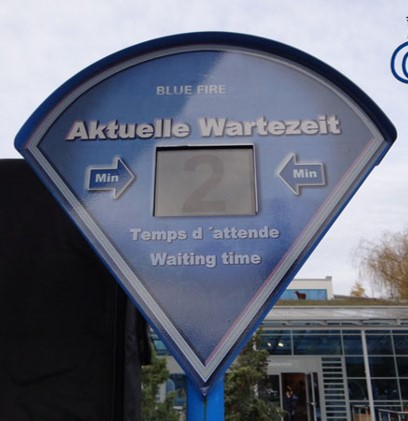
\includegraphics[width=0.4\textwidth]{img/motivation/wartezeit_2.jpg}
    \end{minipage}
    \begin{minipage}{0.49\textwidth}
        \centering
        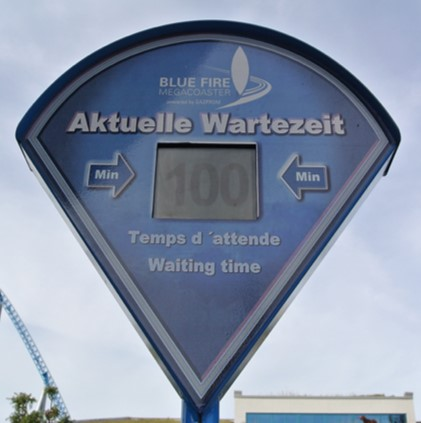
\includegraphics[width=0.4\textwidth]{img/motivation/wartezeit_100.jpg}
    \end{minipage}
\caption[Wartezeitanzeige im Park]{Wartezeitanzeige mit geringer (links) und hoher Wartezeit (rechts)\footnotemark}
		\label{figure:grundlagenwaittime}
\end{figure}
\footnotetext{Bildquellen: \url{http://photobucket.com/gallery/user/Parksonline/media/cGF0aDovMTUtMV96cHM2NjdiYWYxYy5qcGc=/?ref=}, \url{https://www.coasterfriends.de/forum/attachments/eure-tripreports-unsere-freude/240493d1382869532-europa-park-am-26-10-2013-dsc_4001.jpg}}

Der Nachteil daran ist, dass die Wartezeiten  nur direkt beim Betreten der Attraktion sichtbar sind. Es wäre für den Besucher besser, diese auch andernorts und vergleichend betrachten zu können, um besser voraus planen zu können. Auch dafür haben einige Parks eine Lösung gefunden. So gibt es zum Beispiel Monitore mit allen Wartezeiten im Park oder eine parkeigene App mit allen aktuellen Wartezeiten. 

%Bilder Wartezeitübersicht
\begin{figure}[h]
    \centering
    \begin{minipage}{0.49\textwidth}
        \centering
        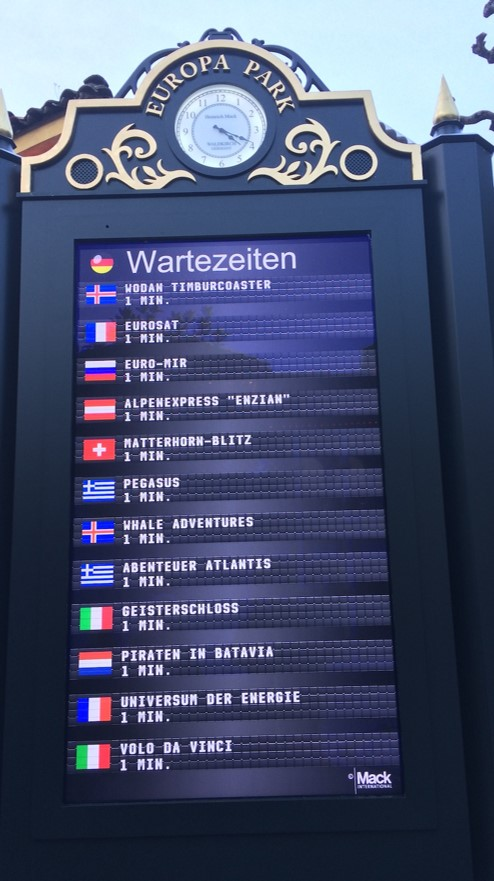
\includegraphics[width=0.4\textwidth]{img/motivation/wartezeit_anzeige.jpg}
    \end{minipage}
    \begin{minipage}{0.49\textwidth}
        \centering
        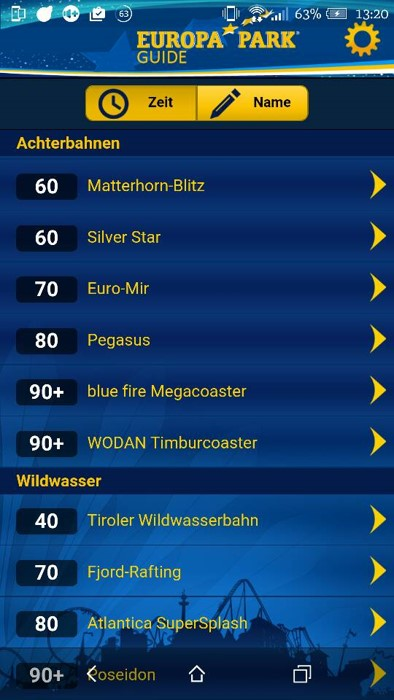
\includegraphics[width=0.4\textwidth]{img/motivation/app_official.jpg}
    \end{minipage}
\caption[Wartezeitübersicht im Europapark]{Wartezeitübersicht des Europaparks als Monitor (links) und als App (rechts)\footnotemark}
		\label{figure:grundlagenwaittime2}
\end{figure}
\footnotetext{Bildquellen: \url{https://www.ep-board.de/download/file.php?id=31185&mode=view}, \url{http://uploads.tapatalk-cdn.com/20160506/d8e6e2c4c8bfc31c9dee0dc32399515a.jpg}}

Da diese parkeigenen Apps, aus verschiedenen Gründen, nur innerhalb des Parks funktionieren, bleibt auch hier das Problem, dass die aktuellen Wartezeiten nur innerhalb des Parks verfügbar sind und man nicht von außerhalb seinen Freizeitparkbesuch planen kann. Es kommt hinzu, dass man meistens nur eine aktuelle Wartezeit zur Verfügung hat, gerne aber weitere Informationen wie die Durchschnitte bestimmter Tage oder Uhrzeiten hätte. Außerdem gibt es bisher kein direktes Feedback der Nutzer über ihre tatsächlich verbrachte Wartezeit. 

Um all diese Probleme zu behben gibt es in unserer App verschiedene Metriken zum Vergleichen der Wartezeiten verschiedener Attraktionen. Diese werden nicht von den Freizeitparks zur Verfügung gestellt, sondern von den Nutzern selbst eingetragen, um somit aus der Gesamtheit aller Nutzerdaten verschiedene Werte berechnen zu können. Speziell unterscheidet unsere App zwischen folgenden fünf Arten von Wartezeiten einer Attraktion:
\begin{itemize}
\item Aktuelle Wartezeit: der Durchschnitt der neusten eingetragen Wartezeiten einer Attraktion, denkbar wäre hier auch das Einbinden von Livedaten aus vorhandenen APIs bestimmter Freizeitparks
\item Tagesdurchschnitt: der Durchschnitt aller eingetragenen Wartezeiten des aktuellen Tages einer Attraktion
\item Gesamtdurchschnitt: der Durchschnitt aller eingetragenen Wartezeiten einer Attraktion
\item Durchschnitt nach Uhrzeit: der Durchschnitt aller eingetragenen Wartezeiten einer Attraktion eines bestimmten Zeitraums
\item Wartezeitenliste: das Anzeigen aller eingetragenen Wartezeiten, welche nach Datum oder Dauer sortiert werden können
\end{itemize}

Da nicht nur die Wartezeit sondern auch die Qualität einer Attraktion ausschlaggebend ist, gibt es in unserer App zusätzlich ein Bewertungssystem für die einzelnen Attraktionen und auch für den Park insgesamt. Dieses ist wie jedes klassische Bewertungssystem durch das "5-Sterne-Bewertungssystem"{} realisiert. Dabei entsprechen 5 Sterne einer hervorragenden und 0 Sterne einer mangelhaften Bewertung.

% Abschnitt: Mobile Plattform
\section{Mobile Plattform Android}
\label{sec:grundlagen:plattforml}

Android ist ein mobiles Betriebssystem, also für Smartphones und Tablets, das von Google entwickelt wurde und auf Linux basiert. Die App-Entwicklung ist geprägt durch einzelne Aktivitäten (ein angezeigter Screen ist eine Aktivität), die miteinander kommunizieren und in ihrer "Lebenszeit"{} ein vorgegebenes Zustandmodell wie in Abbildung \ref{figure:androidZustandsmodell} durchlaufen. Wir beschränken uns in Bezug auf die Plattform Android auf diese kurze Einführung, da die Plattform dank seiner weltweit hohen Verbreitung als bekannt angesehen werden dürfte.

\begin{figure}[htp]
	\centering
  	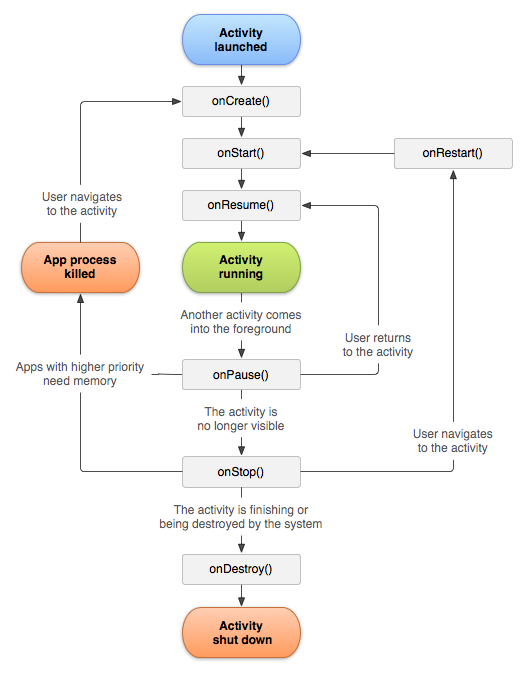
\includegraphics[width=0.5\textwidth]{img/modelle/AndroidZustandsmodell.png}
	\caption[Android Zustandsmodell]{Android Zustandsmodell\footnotemark}
	\label{figure:androidZustandsmodell}
\end{figure}

Ein Nachteil, der während der Entwicklung aufgetreten ist, sind die vielen verschiedenen Android-Versionen und Geräte. Da wir unsere App für so viele Versionen wie möglichen entwickeln wollten, kamen deshalb auch mal das ein oder andere Problem auf, wie z. B. dass manche Libraries oder Frameworks erst ab bestimmten Versionen verfügbar sind oder die vielen verschiedenen Geräte alle unterschiedlichen Seiten- und Größenverhältnisse haben.
\footnotetext{Bildquelle: \url{https://developer.android.com/images/activity_lifecycle.png}}

Die Vorteile von Android überwiegen aber auf jeden Fall, vor allem, wenn man sich damit tiefer beschäftigt und eingearbeitet hat. Einer der größten Vorteile ist die sehr gute Dokumentation von Android durch die das Einlesen in die Möglichkeiten und Funktionen recht leicht ist. Auch die weltweite Verbreitung und Beliebtheit von Android ist hier ein Vorteil, da es sehr viele Entwickler gibt und so jedes Problem schon eimal aufgetreten ist und daher auch zu den allermeisten auch Lösungen oder Workarounds bekannt sind. Außerdem wird Android stetig Weiterentwickelt, weshalb immer mehr möglich ist und der Umgang mit bestimmten Funktionen, wie z. B. der Zugriff auf Gerätefunktionen wie Kamera oder GPS immer leichter wird. Weitere Vorteile für uns sind die Vertrautheit mit Java und die Einfachheit von Android Studio, welches wir für die Entwicklung unserer App benutzt haben.

% Abschnitt: Frameworks
\section{Frameworks}
\label{sec:grundlagen:frameworks}
Frameworks sind eine Art Gerüst oder Rahmen, die eingesetzt werden um das Programmieren zu vereinfachen und die geschriebenen Zeilen zu verringern. Wir haben in unserer App die folgenden aufgelisteten Frameworks als Hilfen genutzt. Alle sind öffentlich und über den jeweiligen Namen auffindbar.
\begin{itemize}
\item Microsoft Azure Mobile App Service: Server mit persistenter Speicherung in SQLite-Datenbank (näheres dazu in Kapitel \ref{sec:implementierung:besonderheiten:azure})
\item Google Firebase: einfache Nutzerverwaltung (näheres dazu in Kapitel \ref{sec:implementierung:besonderheiten:firebase})
\item Cloudinary: kostenloses Hosten und Auslesen von Bildern via HTTP-Request
\item Picasso: erlaubt einfaches Handling (z. B. Größentransformationen) von Bildern in oftmals einer Zeile
\item Glide: ermöglicht eine bessere Darstellung der animierten Lade-Animation
\item MPAndroidCharts: ermöglicht die Erstellung von Diagrammen (in unserem Fall Säulendiagramme für die Statistiken)
\item MaterialChipsInput: Darstellung der Unterkategorien als Chips
\end{itemize}




















\newcommand{\reqtable}[3]{
	\vspace{-1cm}
    \begin{center}
    \begin{tabular}{ | l | p{13cm} |}
    \hline
    \textbf{ID:} & \textbf{#1} \\ \hline
    TITEL: & #2 \\ \hline
    BES: & #3 \\
    \hline
    \end{tabular}
    \end{center}
}

\chapter{Anforderungsanalyse}	
\label{cha:anforderungsanalyse}
In diesem Kapitel werden die ursprünglich definierten funktionalen und nichtfunktionalen Anforderungen tabellarisch dargestellt. Jede der Anforderungen hat einen eindeutigen Identifikator (ID), einen Titel (TITEL), und eine Beschreibung (BES).

% Abschnitt: Funktionale Anforderungen
\section{Funktionale Anforderungen}
\label{sec:anforderungsanalyse:funktional}

\reqtable{FA1}{Startbildschirm}{Nach dem Start der Anwendung sieht der Benutzer einen 
Startbildschirm, auf dem er sich anmelden bzw. registrieren kann, oder ohne Anmeldung zur 
Parkübersicht gelangt.}

\reqtable{FA2}{Parkübersicht}{Diese Ansicht zeigt eine Liste aller Parks, die auf verschiedene 
Weisen sortiert werden kann. Außerdem gibt es eine getrennte Liste, in der sich die favorisierten 
Parks des Nutzers befinden. Sofern die Position des Smartphones bekannt ist, wird die Entfernung 
neben den Parks angezeigt und die Liste kann nach Entfernung sortiert werden.}

\reqtable{FA3}{Park Detailansicht}{Für jeden Park gibt es eine Detailansicht mit näheren 
Informationen. Hier befinden sich Links/Buttons zu den Bewertungen, der Kartenansicht, sowie zur 
Attraktionsübersicht des Parks. Außerdem kann der Park zu den Favoriten hinzugefügt werden.}

\reqtable{FA4}{Bewertungsseite (Park / Attraktionen)}{Es gibt eine Ansicht der neuesten Bewertungen 
(nach Datum sortiert). Eine Bewertung hat jeweils Verfasser, Datum, Stern-Anzahl, und Kommentar. 
Falls der Benutzer eingeloggt ist, sieht er einen Button zum Hinzufügen einer Bewertung.}

\reqtable{FA5}{Bewertung verfassen}{Sofern eingeloggt, kann der Benutzer in einem separaten Dialog 
eine Bewertung verfassen. Hat er zuvor schon eine Bewertung zu diesem Park / dieser Attraktion 
verfasst, kann er diese bearbeiten. Der Administrator kann den Kommentar ausblenden.}

\reqtable{FA6}{Attraktionsübersicht}{Diese Ansicht zeigt eine Liste aller Attraktionen, die auf 
verschiedene Weisen sortiert und gefiltert werden kann. Außerdem gibt es eine getrennte Liste, in 
der sich die favorisierten Attraktionen des Nutzers befinden. Neben jeder Attraktion wird, sofern 
verfügbar, die jeweilige „aktuelle“ Wartezeit angezeigt. (Sofern die Position des Smartphones 
bekannt ist, wird die Entfernung neben den Parks angezeigt und die Liste kann nach Entfernung 
sortiert werden.)}

\reqtable{FA7}{Attraktion Detailansicht}{Für jede Attraktion gibt es eine Detailansicht mit näheren 
Informationen. Hier befinden sich Links/Buttons zu den Bewertungen, der Kartenansicht, sowie zu den 
Wartezeiten. Auch kann die Attraktion zu den Favoriten hinzugefügt werden. Zudem gibt es 
verschiedene Statistiken zu den Wartezeiten (siehe FA8). Ist der Nutzer eingeloggt und befindet 
sich in der Nähe des Parks (GPS muss aktiviert sein), so kann er eine Wartezeit eintragen. Dies 
kann er nur ein Mal pro Stunde machen.}

\reqtable{FA8}{Wartezeit-Statistiken}{Es gibt vier verschiedene Statistiken über die Wartezeit bei 
einer Attraktion:
\begin{itemize}
	\item „Aktuell“: Zeigt die aktuelle Wartezeit an
	\item „Heute“: Zeigt den Durchschnitt für den aktuellen Tag an
	\item „Gesamt“: Zeigt den bisherigen Gesamtdurchschnitt an
	\item Ein Säulendiagramm, welches den stündlichen bisherigen Durchschnitt anzeigt
\end{itemize}
}

\reqtable{FA9}{Wartezeitenverlauf}{Es gibt eine Listenansicht der bisher eingetragenen Wartezeiten 
einer Attraktion. Ein Wartezeiten-Eintrag enthält Verfasser, Datum, Uhrzeit und Wartezeit (in 
Minuten).}

\reqtable{FA10}{Admin-Funktionen}{Ein Administrator hat folgende Zusatzfunktionen:
\begin{itemize}
\item Parks / Attraktionen hinzufügen und erstellte bearbeiten
\item Kommentare ausblenden
\end{itemize}
}

% Abschnitt: Nichtfunktionale Anforderungen
\section{Nichtfunktionale Anforderungen}
\label{sec:anforderungsanalyse:nichtfunktional}

\reqtable{NFA1}{Entwicklungssprache und -umgebung}{Die Anwendung wird in Java mit der 
Entwicklungsumgebung „Android Studio“ entwickelt und soll auf Geräten mit Betriebssystemen ab 
Android 4.1 funktionieren.}

\reqtable{NFA2}{Reaktionszeit}{Die Reaktionszeit der Anwendung soll zu jeder Zeit maximal 1,5 
Sekunden betragen}

\reqtable{NFA3}{Benutzbarkeit}{Die Anwendung soll intuitiv bedienbar sein. D.h., die Buttons und 
andere Auswahlmöglichkeiten sollen eine ausreichende Größe haben und wie erwartet reagieren.}

\reqtable{NFA4}{Offline-Modus}{Die Anwendung soll alle Anfragen zwischenspeichern, um auch Offline 
Zugriff auf die wichtigen Informationen zu gewährleisten (Bilder werden von der Bild-Bibliothek 
gecached).}
%\chapter{Konzept und Entwurf}

Wie üblich bei einem Projekt startet man mit Mockups der Anwendung, damit der Kunde eine genauere Vorstellung seiner Ideen bekommt. 

Wir haben uns ziemlich stark an unsere Mockups gehalten und im Folgenden sieht man jedes Mockup gepaart mit dem dazugehörigen Screenshot aus der fertigen App.

Wenn man die App öffnet befindet man sich als erstes auf der Startseite.\\

\begin{figure}[h]
    \centering
    \begin{minipage}{0.45\textwidth}
        \centering
        \includegraphics[width=0.75\textwidth]{img/mockups/main_screen.png}
        \caption{first figure}
    \end{minipage}
    \begin{minipage}{0.45\textwidth}
        \centering
        \includegraphics[width=0.75\textwidth]{img/screenshots/device_main_screen.png}
        \caption{second figure}
    \end{minipage}
\end{figure}

Als nächstes manövriert man zu einem neuen Spiel. Hier haben wir, anders als in dem Mockup, die Einstellungen nur angezeigt, aber man kann sie natürlch noch ändern bevor man das Spiel startet. Ein Deck muss aber jedes mal gewählt werden. \\

\begin{figure}[h]
    \centering
    \begin{minipage}{0.45\textwidth}
        \centering
        \includegraphics[width=0.4\textwidth]{img/mockups/neues_spiel.png}
        \caption{first figure}
    \end{minipage}\hfill
    \begin{minipage}{0.45\textwidth}
        \centering
        \includegraphics[width=0.4\textwidth]{img/screenshots/device_new_game.png}
        \caption{second figure}
    \end{minipage}
\end{figure}

Will man jetzt doch noch etwas an den Einstellungen ändern, tippt man auf Einstellungen anpassen und kann nun beliebig Anpassungen vornehmen.

\begin{figure}[h]
    \centering
    \begin{minipage}{0.45\textwidth}
        \centering
        \includegraphics[width=0.4\textwidth]{img/mockups/einstellungen.png}
        \caption{first figure}
    \end{minipage}\hfill
    \begin{minipage}{0.45\textwidth}
        \centering
        \includegraphics[width=0.4\textwidth]{img/screenshots/device_settings.png}
        \caption{second figure}
    \end{minipage}
\end{figure}

\chapter{Konzept, Entwurf und Implementierung}
\label{cha:implementierung}

% Abschnitt: Implementierungsdetails
\section{Implementierungsdetails}
\label{sec:implementierung:implementierungsdetails}

TODO

%Bildervorlage
\begin{figure}[h]
    \centering
    \begin{minipage}{0.49\textwidth}
        \centering
        
\includegraphics[width=0.4\textwidth]{img/coaster42_logo.png}
        \caption{Hauptmenü der App}
		\label{figure:implementierungmenue}
    \end{minipage}
    \begin{minipage}{0.49\textwidth}
        \centering
        
\includegraphics[width=0.4\textwidth]{img/coaster42_logo.png}
        \caption{Mockup Hauptmenü}
    \end{minipage}
\end{figure}



% Abschnitt: Besonderheiten 
\section{Besonderheiten}
\label{sec:implementierung:besonderheiten }

TODO

\subsection{Wartezeit berechung und -darstellung}
\label{sec:implementierung:besonderheiten:wartezeit }

\subsection{Client-Server-Kommunikation mit Azure}
\label{sec:implementierung:besonderheiten:azure }

%Download- und Upload-Verlauf-Modell

\subsection{User-Verwaltung mit Firebase}
\label{sec:implementierung:besonderheiten:firebase }

%Firebase Modell?

\subsection{Adminfunktionen}
\label{sec:implementierung:besonderheiten:admin }



% Abschnitt: Architektur
\section{Architektur}
\label{sec:implementierung:architektur}

\subsection{Datenmodell und -speicherung}
\label{sec:implementierung:architektur:datenmodell }

TODO

\subsection{Klassen- und Activity-Architektur}
\label{sec:implementierung:architektur:klassenmodell }

TODO

\subsection{Arbeitsaufteilung}
\label{sec:implementierung:architektur:arbeitsaufteilung }

Während der Implementation wurden die Aufgaben so aufgeteilt, dass jeder aus dem Team immer für eine bestimmte Aufgabe zuständig war und diese durch alle Schichten durch erledigen musste. Bei großen Aufgaben, wie dem Spielablauf, wurden die Aufgabe zudem in kleinere Schritte aufgeteilt. Da die App aus mehreren unabhängigen Bereichen besteht, konnten die Aufgaben gut eingeteilt werden, ohne dass es zu Behinderungen kommt. Wenn gerade keine Arbeit für eine Person angefallen war, beschäftigte diese sich mit Verbesserungen, Testen von Funktionen oder mit der Weiterentwicklung des Designs.

% Abschnitt: Schwierigkeiten während der Implementierung 
\section{Schwierigkeiten während der Implementierung}
\label{sec:implementierung:schwierigkeiten }	

TODO

\begin{itemize} 
\item 1
\item 2
\end{itemize}





% tabellenzeile dreispaltig
\newcommand{\td}[3]{
	#1 & #2 & #3 \\ \hline
}

\chapter{Anforderungsabgleich}
\label{cha:anforderungsabgleich}

Es folgt ein tabellarischer Vergleich zwischen den in Kapitel \ref{cha:anforderungsanalyse} 
spezifizierten Anforderungen und den implementierten Funktionen. Es wird für jede der Anforderungen 
beurteilt, inwieweit diese in der Implementierung erfüllt ist (Ja / Teilweise / Nein). Eine 
Zuordnung zu den Einträgen aus Kapitel \ref{cha:anforderungsanalyse} ist anhand der ID möglich.

Diejenigen Funktionen, die implementiert wurden, jedoch nicht im Voraus als Anforderungen 
spezifiziert waren, werden in diesem Vergleich nicht berücksichtigt.

\clearpage

\label{sec:anforderungsabgleich:funktional}
\label{sec:anforderungsabgleich:nichtfunktional}

% padding anpassen für tabelle
\setlength{\tabcolsep}{10pt}
\renewcommand{\arraystretch}{1.3}

\begin{center}
	\begin{table}[h]
		\begin{tabular}{ | l | l | p{11.5cm} |}
			%TODO Breite automatisch die Seite füllen lassen? (\textwidth ist zu lang)
			%Beide Tabellen wurden zu einer zusammen geführt, damit Inhaltsverzeichnis auf eine Seite passt :D
			\hline
			\textbf{ID} & \textbf{Erfüllt} & \textbf{Kommentar} \\ \hline
			\td{FA1}{Nein}{Unnötig, da die Account-Funktionen im Sidebar-Menü untergebracht wurden 
			und die Anwendung direkt auf der Parkübersicht startet.}
			\td{FA2}{Ja}{-}
			\td{FA3}{Ja}{-}
			\td{FA4}{Ja}{-}
			\td{FA5}{Ja}{-}
			\td{FA6}{Ja}{-}
			\td{FA7}{Ja}{-}
			\td{FA8}{Ja}{Es sind weiterhin 4 verschiedene Statistiken, jedoch wurde die Semantik 
			leicht geändert, um sie hilfreicher zu machen (siehe Kapitel 4.2.1 
			``Wartezeit-Berechnung und -darstellung'').}
			\td{FA9}{Ja}{-}
			\td{FA10}{Ja}{-}
			\td{NFA1}{Ja}{-}
			\td{NFA2}{Ja}{Die Zeit zum Hoch- oder Herunterladen von Daten liegt je nach Qualität der 
			Internetverbingung unter oder weit über 1,5 Sekunden, aber dieser Vorgang blockiert nicht 
			die Benutzeroberfläche und kann abgebrochen werden. Dank der Offline-Daten gibt es aber 
			nie lange Ladezeiten innerhalb der App.}
			\td{NFA3}{Ja}{Die Anforderung ist nur schwer zu beurteilen. Es wurde sich möglichst an die 
			Android-Richtlinien für Benutzeroberflächen gehalten, und alle Bereiche der 
			Anwendung sind nach dem Empfinden aller bisherigen Benutzer leicht bedienbar.}
			\td{NFA4}{Ja}{-}
		\end{tabular}
	\end{table}
\end{center}

% padding wieder auf standard
\setlength{\tabcolsep}{6pt}
\renewcommand{\arraystretch}{1}



\chapter{Ausblick}
\label{cha:Ausblick}

Wie im Kapitel \ref{cha:anforderungsabgleich} zu sehen ist, haben wir all unsere inhaltlichen Anforderungen an die App erfüllt. Deswegen haben wir uns in diesem Kapitel einige Gedanken gemacht, welche Funktionen  für eine zukünftige Erweiterung der App denkbar wären. Diese könnten die bisherigen Funktionen sinnvoll ergänzen.

\begin{itemize}
\item Wartezeitenverifizierung: Bisher gibt es in unserer App keine Möglichkeit, falsch eingetragene Wartezeiten zu melden oder rückgängig zu machen. Zwar gleichen sich einzelne falsch eingetragene Wartezeiten dank der verwendeten Metriken zur Berechnung der Durchschnittswartezeiten schnell aus und haben keinen großen Einfluss. Trotzdem wäre es eine gute Ergänzung, wenn andere Nutzer die zuletzt eingetragenen Wartezeiten bestätigen oder ablehnen könnten, sodass die jeweilige Wartezeit an Gewichtung zu- oder abnimmt.
\item Ansteh-Timer: Um die Wartezeit nicht jedes mal selbst messen oder ablesen zu müssen, wäre ein Ansteh-Timer eine gute Ergänzung für die Benutzer der App. Dazu wird beim Beginn des Anstehens ein Startknopf gedrückt, welcher den Timer startet. Kurz vor der Fahrt oder direkt nach der Fahrt kann dann der Stoppknopf gedrückt werden. Dadurch wird die gewartete Zeit automatisch ermittelt und hochgeldaen.
\item Bewertungskategorisierung: Bisher gibt es bei unseren Bewertungen für die Parks und Attraktionen jeweils nur die Möglichkeit, allgemein zwischen null und fünf Sternen zu verteilen. Noch besser wäre, für jeden Park oder jede Attraktion bestimmte Kriterien der Kategorisierung vorzunehmen. So könnten zum Beispiel Achterbahnen nach der Action, Wasserbahnen nach ihrer Erfrischung, Familienbahnen nach der Tauglichkeit für Kinder oder Restaurants nach dem Geschmack bewertet werden. Dies bietet sich besonders bei Attraktionen an, da sie zum einen bereits in verschiedene Kategorien aufgeteilt sind. Zum anderen laufen die Benutzer so nicht in Gefahr, zum Beispiel eine Kinderbahn niedriger zu bewerten, weil sie nicht genügend Action für sie bereit hält.
\item Tourplaner: Da die Attraktionen schon in einer Mapview angezeigt werden, wäre es eine sinnvolle Ergänzung, den Benutzern die Möglichkeit zu geben, sich selbst eine Tour zusammen zu stellen, welche sie dann auf der Karte angezeigt bekommen. Desweiteren könnten auch bereits vorhandene Touren geladen werden oder Touren automatisch erstellt werden, zum Beispiel nach Kategorien oder nach Wartezeiten.
\end{itemize}

Zudem besteht zumindest theoretisch die Möglichkeit, Freizeitparks und ihre Daten direkt mit in die App einzubinden. Dadurch ergibt sich auch die Möglichkeit, wie sich die App finanzieren könnte. Freizeitparks, die eine Kooperation eingehen, könnten Vorteile oder Premiumaccounts erhalten. Mögliche Vorteile wären neben dem selbstständigen Verwalten der eigenen Parkdaten zum Beispiel das Einbinden ihrer eigenen Live-Wartezeiten aus bereits vorhandenen parkeigenen APIs, das Schalten von Werbung oder Aktionen des Freizeitparks oder auch das Hervorheben des Freizeitparks durch ein besonderes Design oder eine gut sichtbare Platzierung in der Übersichtsliste. 

\chapter{Fazit}
\label{cha:Fazit}

In diesem Kapitel soll ein kurzes Fazit zur App-Entwicklung und zum Anwendungsfach allgemein festgehalten werden.

Dadurch, dass wir als Team schon im Semester zuvor die Quartett-App zusammen entwickelt haben, hatten wir schon genügend Vorwissen, um in die Entwicklung unserer Freizeitpark-App einzusteigen. Trotzdem haben wir auch während der Entwicklung dieser App viel Neues gelernt was wir für die Zukunft und für die Entwicklung weiterer Apps gebrauchen können, wie zum Beispiel das Arbeiten mit Standorten und das Einbinden von vorhandenen Frameworks.

In unseren Augen ist uns die Coaster2Go App größtenteils gut gelungen und das Endergebnis ist genau so, wie wir es uns am Anfang des Semesters vorgestellt haben. Die App wäre theoretisch schon ausreichend für eine Veröffentlichung im App Store, da es bisher keine vergleichbare App im Google Play Store gibt. Natürlich gäbe es noch einige Stellen, die eine Anpassung benötigen, bevor es wirklich zu einer Veröffentlichung kommen kann. Zum Beispiel müsste die Speicherung der Daten auf einen anderen Server verlegt werden, da wir bisher mit unseren Studentenaccounts nur begrenzte Kapazitäten besitzen. Auch kleinere gestalttechnische oder funktionale Verbesserungen sind denkbar. 

Auch was das Arbeiten im Team und die Aufteilung der Aufgaben angeht, konnten wir im Vergleich zum ersten Teil des Anwendungsfaches noch Neues dazu lernen. Die Teamarbeit hat immer gut funktioniert und es kam nie zu größeren Komplikationen. Wir werden es auf jeden Fall in Erwägung ziehen, möglicherweise im Masterstudium das Anwendungsfach fortzusetzen.


% Bibliograhpy
\bibliographystyle{splncs}
\begingroup
\interlinepenalty 10000
\sloppy
\bibliography{literature}
\endgroup

% anhänge
%\appendix
% hier kommen die anhänge
%\chapter{Quelltexte}

In diesem Anhang sind einige wichtige Quelltexte aufgeführt.

\begin{lstlisting}[caption={Zeilencode}]
public class Hello {
    public static void main(String[] args) {
        System.out.println("Hello World");
    }
}
\end{lstlisting}


\backmatter			% abtrennung für verzeichnisse

% hier die verzeichnisse
\listoffigures
%\listoftables


\clearpage
%\erklaerung

\end{document}
